% Options for packages loaded elsewhere
\PassOptionsToPackage{unicode}{hyperref}
\PassOptionsToPackage{hyphens}{url}
\PassOptionsToPackage{dvipsnames,svgnames,x11names}{xcolor}
%
\documentclass[
  letterpaper,
  DIV=11,
  numbers=noendperiod]{scrartcl}

\usepackage{amsmath,amssymb}
\usepackage{iftex}
\ifPDFTeX
  \usepackage[T1]{fontenc}
  \usepackage[utf8]{inputenc}
  \usepackage{textcomp} % provide euro and other symbols
\else % if luatex or xetex
  \usepackage{unicode-math}
  \defaultfontfeatures{Scale=MatchLowercase}
  \defaultfontfeatures[\rmfamily]{Ligatures=TeX,Scale=1}
\fi
\usepackage{lmodern}
\ifPDFTeX\else  
    % xetex/luatex font selection
\fi
% Use upquote if available, for straight quotes in verbatim environments
\IfFileExists{upquote.sty}{\usepackage{upquote}}{}
\IfFileExists{microtype.sty}{% use microtype if available
  \usepackage[]{microtype}
  \UseMicrotypeSet[protrusion]{basicmath} % disable protrusion for tt fonts
}{}
\makeatletter
\@ifundefined{KOMAClassName}{% if non-KOMA class
  \IfFileExists{parskip.sty}{%
    \usepackage{parskip}
  }{% else
    \setlength{\parindent}{0pt}
    \setlength{\parskip}{6pt plus 2pt minus 1pt}}
}{% if KOMA class
  \KOMAoptions{parskip=half}}
\makeatother
\usepackage{xcolor}
\setlength{\emergencystretch}{3em} % prevent overfull lines
\setcounter{secnumdepth}{-\maxdimen} % remove section numbering
% Make \paragraph and \subparagraph free-standing
\makeatletter
\ifx\paragraph\undefined\else
  \let\oldparagraph\paragraph
  \renewcommand{\paragraph}{
    \@ifstar
      \xxxParagraphStar
      \xxxParagraphNoStar
  }
  \newcommand{\xxxParagraphStar}[1]{\oldparagraph*{#1}\mbox{}}
  \newcommand{\xxxParagraphNoStar}[1]{\oldparagraph{#1}\mbox{}}
\fi
\ifx\subparagraph\undefined\else
  \let\oldsubparagraph\subparagraph
  \renewcommand{\subparagraph}{
    \@ifstar
      \xxxSubParagraphStar
      \xxxSubParagraphNoStar
  }
  \newcommand{\xxxSubParagraphStar}[1]{\oldsubparagraph*{#1}\mbox{}}
  \newcommand{\xxxSubParagraphNoStar}[1]{\oldsubparagraph{#1}\mbox{}}
\fi
\makeatother

\usepackage{color}
\usepackage{fancyvrb}
\newcommand{\VerbBar}{|}
\newcommand{\VERB}{\Verb[commandchars=\\\{\}]}
\DefineVerbatimEnvironment{Highlighting}{Verbatim}{commandchars=\\\{\}}
% Add ',fontsize=\small' for more characters per line
\usepackage{framed}
\definecolor{shadecolor}{RGB}{241,243,245}
\newenvironment{Shaded}{\begin{snugshade}}{\end{snugshade}}
\newcommand{\AlertTok}[1]{\textcolor[rgb]{0.68,0.00,0.00}{#1}}
\newcommand{\AnnotationTok}[1]{\textcolor[rgb]{0.37,0.37,0.37}{#1}}
\newcommand{\AttributeTok}[1]{\textcolor[rgb]{0.40,0.45,0.13}{#1}}
\newcommand{\BaseNTok}[1]{\textcolor[rgb]{0.68,0.00,0.00}{#1}}
\newcommand{\BuiltInTok}[1]{\textcolor[rgb]{0.00,0.23,0.31}{#1}}
\newcommand{\CharTok}[1]{\textcolor[rgb]{0.13,0.47,0.30}{#1}}
\newcommand{\CommentTok}[1]{\textcolor[rgb]{0.37,0.37,0.37}{#1}}
\newcommand{\CommentVarTok}[1]{\textcolor[rgb]{0.37,0.37,0.37}{\textit{#1}}}
\newcommand{\ConstantTok}[1]{\textcolor[rgb]{0.56,0.35,0.01}{#1}}
\newcommand{\ControlFlowTok}[1]{\textcolor[rgb]{0.00,0.23,0.31}{\textbf{#1}}}
\newcommand{\DataTypeTok}[1]{\textcolor[rgb]{0.68,0.00,0.00}{#1}}
\newcommand{\DecValTok}[1]{\textcolor[rgb]{0.68,0.00,0.00}{#1}}
\newcommand{\DocumentationTok}[1]{\textcolor[rgb]{0.37,0.37,0.37}{\textit{#1}}}
\newcommand{\ErrorTok}[1]{\textcolor[rgb]{0.68,0.00,0.00}{#1}}
\newcommand{\ExtensionTok}[1]{\textcolor[rgb]{0.00,0.23,0.31}{#1}}
\newcommand{\FloatTok}[1]{\textcolor[rgb]{0.68,0.00,0.00}{#1}}
\newcommand{\FunctionTok}[1]{\textcolor[rgb]{0.28,0.35,0.67}{#1}}
\newcommand{\ImportTok}[1]{\textcolor[rgb]{0.00,0.46,0.62}{#1}}
\newcommand{\InformationTok}[1]{\textcolor[rgb]{0.37,0.37,0.37}{#1}}
\newcommand{\KeywordTok}[1]{\textcolor[rgb]{0.00,0.23,0.31}{\textbf{#1}}}
\newcommand{\NormalTok}[1]{\textcolor[rgb]{0.00,0.23,0.31}{#1}}
\newcommand{\OperatorTok}[1]{\textcolor[rgb]{0.37,0.37,0.37}{#1}}
\newcommand{\OtherTok}[1]{\textcolor[rgb]{0.00,0.23,0.31}{#1}}
\newcommand{\PreprocessorTok}[1]{\textcolor[rgb]{0.68,0.00,0.00}{#1}}
\newcommand{\RegionMarkerTok}[1]{\textcolor[rgb]{0.00,0.23,0.31}{#1}}
\newcommand{\SpecialCharTok}[1]{\textcolor[rgb]{0.37,0.37,0.37}{#1}}
\newcommand{\SpecialStringTok}[1]{\textcolor[rgb]{0.13,0.47,0.30}{#1}}
\newcommand{\StringTok}[1]{\textcolor[rgb]{0.13,0.47,0.30}{#1}}
\newcommand{\VariableTok}[1]{\textcolor[rgb]{0.07,0.07,0.07}{#1}}
\newcommand{\VerbatimStringTok}[1]{\textcolor[rgb]{0.13,0.47,0.30}{#1}}
\newcommand{\WarningTok}[1]{\textcolor[rgb]{0.37,0.37,0.37}{\textit{#1}}}

\providecommand{\tightlist}{%
  \setlength{\itemsep}{0pt}\setlength{\parskip}{0pt}}\usepackage{longtable,booktabs,array}
\usepackage{calc} % for calculating minipage widths
% Correct order of tables after \paragraph or \subparagraph
\usepackage{etoolbox}
\makeatletter
\patchcmd\longtable{\par}{\if@noskipsec\mbox{}\fi\par}{}{}
\makeatother
% Allow footnotes in longtable head/foot
\IfFileExists{footnotehyper.sty}{\usepackage{footnotehyper}}{\usepackage{footnote}}
\makesavenoteenv{longtable}
\usepackage{graphicx}
\makeatletter
\newsavebox\pandoc@box
\newcommand*\pandocbounded[1]{% scales image to fit in text height/width
  \sbox\pandoc@box{#1}%
  \Gscale@div\@tempa{\textheight}{\dimexpr\ht\pandoc@box+\dp\pandoc@box\relax}%
  \Gscale@div\@tempb{\linewidth}{\wd\pandoc@box}%
  \ifdim\@tempb\p@<\@tempa\p@\let\@tempa\@tempb\fi% select the smaller of both
  \ifdim\@tempa\p@<\p@\scalebox{\@tempa}{\usebox\pandoc@box}%
  \else\usebox{\pandoc@box}%
  \fi%
}
% Set default figure placement to htbp
\def\fps@figure{htbp}
\makeatother

\KOMAoption{captions}{tableheading}
\makeatletter
\@ifpackageloaded{caption}{}{\usepackage{caption}}
\AtBeginDocument{%
\ifdefined\contentsname
  \renewcommand*\contentsname{Table of contents}
\else
  \newcommand\contentsname{Table of contents}
\fi
\ifdefined\listfigurename
  \renewcommand*\listfigurename{List of Figures}
\else
  \newcommand\listfigurename{List of Figures}
\fi
\ifdefined\listtablename
  \renewcommand*\listtablename{List of Tables}
\else
  \newcommand\listtablename{List of Tables}
\fi
\ifdefined\figurename
  \renewcommand*\figurename{Figure}
\else
  \newcommand\figurename{Figure}
\fi
\ifdefined\tablename
  \renewcommand*\tablename{Table}
\else
  \newcommand\tablename{Table}
\fi
}
\@ifpackageloaded{float}{}{\usepackage{float}}
\floatstyle{ruled}
\@ifundefined{c@chapter}{\newfloat{codelisting}{h}{lop}}{\newfloat{codelisting}{h}{lop}[chapter]}
\floatname{codelisting}{Listing}
\newcommand*\listoflistings{\listof{codelisting}{List of Listings}}
\makeatother
\makeatletter
\makeatother
\makeatletter
\@ifpackageloaded{caption}{}{\usepackage{caption}}
\@ifpackageloaded{subcaption}{}{\usepackage{subcaption}}
\makeatother

\usepackage{bookmark}

\IfFileExists{xurl.sty}{\usepackage{xurl}}{} % add URL line breaks if available
\urlstyle{same} % disable monospaced font for URLs
\hypersetup{
  pdftitle={Adult Income (1994 Census) --- Exploratory Data Analysis},
  pdfauthor={Kwaku Owusu-Tieku},
  colorlinks=true,
  linkcolor={blue},
  filecolor={Maroon},
  citecolor={Blue},
  urlcolor={Blue},
  pdfcreator={LaTeX via pandoc}}


\title{Adult Income (1994 Census) --- Exploratory Data Analysis}
\author{Kwaku Owusu-Tieku}
\date{2026-07-20}

\begin{document}
\maketitle


\section{Introduction}\label{introduction}

This dataset records 32,561 individuals drawn from the 1994 US Current
Population Survey (CPS) by Barry Becker at UC Irvine. Each row describes
a working-age adult's demographic characteristics and whether their
annual income exceeds \$50,000. The dataset was published as a
machine-learning benchmark in the UCI repository, where its original
purpose was binary income classification.

This analysis treats it not as a benchmark but as a window into the US
labor market in 1994 --- who was earning above a threshold equivalent to
roughly \$100,000 in today's dollars, and which structural factors
(education, occupation, marital status, age) tracked most closely with
that outcome. Three questions guide the analysis:

\begin{enumerate}
\def\labelenumi{\arabic{enumi}.}
\tightlist
\item
  Where in the educational hierarchy does high income become the
  \emph{majority} outcome, rather than the exception?
\item
  What does the widely-reported gender income gap actually look like
  once marital status is held constant?
\item
  What does the structure of capital gains in this sample reveal about
  who builds wealth through investment vs.~wage income alone?
\end{enumerate}

\textbf{Domain brief note.} This analysis was conducted for learning and
skill demonstration purposes, without a specific downstream decision or
audience constraint. The analysis proceeds on the analyst's own judgment
about what the data most clearly shows.

\section{The Data}\label{the-data}

\subsection{Source}\label{source}

The underlying data is the \textbf{1994 Census Bureau Current Population
Survey (CPS)}, specifically the ``adult'' extract created by Barry
Becker and Ronny Kohavi and deposited in the UCI Machine Learning
Repository. The CPS is a monthly survey of roughly 60,000 US households
conducted jointly by the Bureau of Labor Statistics and the Census
Bureau; the 1994 extract targets the civilian noninstitutional
population aged 16 and older.

Collection era: \textbf{1994.} \$50,000 in 1994 dollars is equivalent to
approximately \textbf{\$105,800 in 2024 dollars} (BLS CPI-U: annual
index 148.2 in 1994 → 313.7 in 2024). The threshold was not modest: it
sat approximately 60\% above the 1994 male median full-time/year-round
earnings of \$31,609 (Census P60-189), and was more than double the
female median of \$23,261. The SSA national average wage for all covered
workers in 1994 was \$23,754 --- less than half the threshold. In the
actual 1994 labor force, \$50K individual income placed a worker in
roughly the top 20--25\% of earners. Any claim made from this data
should be read in that era context; wage distributions, educational
attainment, and labor force participation have all shifted substantially
in the intervening 30 years.

The dataset does not include a \texttt{year} column --- it is a
cross-sectional extract, not a longitudinal record.

\subsection{Sample Representativeness}\label{sample-representativeness}

The dataset's demographic composition compared against the 1994 civilian
labor force (BLS EcoPro Table 1):

\begin{longtable}[]{@{}llll@{}}
\toprule\noalign{}
Group & Dataset & BLS 1994 & Difference \\
\midrule\noalign{}
\endhead
\bottomrule\noalign{}
\endlastfoot
Female & 33.1\% & 45.9\% & −12.8 pts \\
White & 85.4\% & 84.8\% & +0.6 pts \\
Black & 9.6\% & 11.1\% & −1.5 pts \\
Asian(-Pac-Islander) & 3.2\% & 4.2\% & −1.0 pts \\
Bachelor's or higher & 24.8\% & \textasciitilde24--25\% &
\textasciitilde0 \\
\end{longtable}

\textbf{White racial composition matches the 1994 labor force almost
exactly.} Educational composition also aligns. However, \textbf{the
dataset substantially underrepresents women} --- 33.1\% female
vs.~45.9\% in the actual labor force, a 12.8-point gap. This is
consistent with the CPS sampling frame excluding non-labor-force
participants and potentially reflecting a 1994 extraction methodology
that skewed male. Black and Asian representation are mildly
underrepresented by 1--1.5 points.

The unweighted analyses throughout this report are based on a sample
that underrepresents women by roughly one-eighth. The fnlwgt sampling
weights would correct for this in a weighted analysis; using unweighted
results for gender comparisons means the male perspective is weighted
approximately 2:1 over the female perspective relative to the actual
1994 labor force. This does not invalidate the within-group findings
(e.g., the married-female vs.~married-male comparison) but it does
affect any aggregate female income statistics.

\subsection{Reading the Data}\label{reading-the-data}

\begin{Shaded}
\begin{Highlighting}[]
\NormalTok{df }\OtherTok{\textless{}{-}} \FunctionTok{read\_parquet}\NormalTok{(}\StringTok{"../data/processed/adult\_clean.parquet"}\NormalTok{)}
\end{Highlighting}
\end{Shaded}

\textbf{Column dictionary} (15 columns, no header row in the source file
--- names applied from \texttt{adult.names}):

\begin{longtable}[]{@{}
  >{\raggedright\arraybackslash}p{(\linewidth - 4\tabcolsep) * \real{0.3333}}
  >{\raggedright\arraybackslash}p{(\linewidth - 4\tabcolsep) * \real{0.3333}}
  >{\raggedright\arraybackslash}p{(\linewidth - 4\tabcolsep) * \real{0.3333}}@{}}
\toprule\noalign{}
\begin{minipage}[b]{\linewidth}\raggedright
Column
\end{minipage} & \begin{minipage}[b]{\linewidth}\raggedright
Type
\end{minipage} & \begin{minipage}[b]{\linewidth}\raggedright
Description
\end{minipage} \\
\midrule\noalign{}
\endhead
\bottomrule\noalign{}
\endlastfoot
age & numeric & Age in years; possible top-code at 90 \\
workclass & categorical & Employment sector (Private, Federal-gov,
Self-emp-inc, etc.) \\
fnlwgt & numeric & CPS sampling weight --- how many US adults this row
represents \\
education & ordered categorical & Highest degree attained (Preschool →
Doctorate) \\
education\_num & numeric & Numeric encoding of education (1=Preschool,
16=Doctorate) \\
marital\_status & categorical & 7 categories including three married
variants \\
occupation & categorical & Job type (14 named + missing) \\
relationship & categorical & Household relationship role (Husband, Wife,
etc.) \\
race & categorical & 5 categories \\
sex & categorical & Male / Female \\
capital\_gain & numeric & Annual investment income gain; top-coded at
\$99,999 \\
capital\_loss & numeric & Annual investment income loss \\
hours\_per\_week & numeric & Reported weekly work hours; top-coded at
99 \\
native\_country & categorical & Country of birth; 41 named + missing \\
income & binary & ≤\$50K or \textgreater\$50K \\
\end{longtable}

\section{Data Quality Checks}\label{data-quality-checks}

\subsection{Record Count Verification}\label{record-count-verification}

\begin{Shaded}
\begin{Highlighting}[]
\NormalTok{tbl\_rc }\OtherTok{\textless{}{-}} \FunctionTok{readRDS}\NormalTok{(}\StringTok{"../data/processed/tbl\_record\_count.rds"}\NormalTok{)}
\NormalTok{knitr}\SpecialCharTok{::}\FunctionTok{kable}\NormalTok{(tbl\_rc)}
\end{Highlighting}
\end{Shaded}

\begin{longtable}[]{@{}lrrl@{}}
\toprule\noalign{}
Item & Expected & Actual & Notes \\
\midrule\noalign{}
\endhead
\bottomrule\noalign{}
\endlastfoot
Rows & 32561 & 32561 & Matches documented train-set size \\
\end{longtable}

32,561 rows, exactly matching the documented UCI training-set size. No
discrepancy.

\subsection{Null / Missing Value Check}\label{null-missing-value-check}

The raw file encodes all missing values as the string \texttt{"?"}
rather than true \texttt{NA} --- a disguised-null convention. Three
columns are affected:

\begin{Shaded}
\begin{Highlighting}[]
\NormalTok{tbl\_miss }\OtherTok{\textless{}{-}} \FunctionTok{readRDS}\NormalTok{(}\StringTok{"../data/processed/tbl\_missing.rds"}\NormalTok{)}
\NormalTok{knitr}\SpecialCharTok{::}\FunctionTok{kable}\NormalTok{(tbl\_miss)}
\end{Highlighting}
\end{Shaded}

\begin{longtable}[]{@{}
  >{\raggedright\arraybackslash}p{(\linewidth - 6\tabcolsep) * \real{0.1429}}
  >{\raggedleft\arraybackslash}p{(\linewidth - 6\tabcolsep) * \real{0.0762}}
  >{\raggedleft\arraybackslash}p{(\linewidth - 6\tabcolsep) * \real{0.0952}}
  >{\raggedright\arraybackslash}p{(\linewidth - 6\tabcolsep) * \real{0.6857}}@{}}
\toprule\noalign{}
\begin{minipage}[b]{\linewidth}\raggedright
Column
\end{minipage} & \begin{minipage}[b]{\linewidth}\raggedleft
? count
\end{minipage} & \begin{minipage}[b]{\linewidth}\raggedleft
\% of rows
\end{minipage} & \begin{minipage}[b]{\linewidth}\raggedright
Handling
\end{minipage} \\
\midrule\noalign{}
\endhead
\bottomrule\noalign{}
\endlastfoot
workclass & 1836 & 5.6 & Replaced with NA; kept in dataset; sensitivity
noted \\
occupation & 1843 & 5.7 & Replaced with NA; structurally co-missing with
workclass for 1,836 rows \\
native\_country & 583 & 1.8 & Replaced with NA; kept in dataset;
independent missingness pattern \\
\end{longtable}

\textbf{workclass and occupation are co-missing for 1,836 rows exactly.}
Zero rows have missing workclass without also having missing occupation.
This is structural --- the same respondents who declined to specify
employment sector consistently also left occupation blank. Among these
1,836 rows, only 10.4\% earn \textgreater\$50K, compared to 24.1\% in
the full dataset. Dropping missing rows would mildly oversample
high-income individuals. In this EDA, missing rows are retained with
\texttt{NA} values and excluded from per-group proportions where noted.

\textbf{native\_country missingness is independent.} Only 27 of the 583
missing native\_country rows also have missing workclass --- different
respondents, different pattern, likely different non-response reason.

\subsection{Numeric Range Validation}\label{numeric-range-validation}

\begin{Shaded}
\begin{Highlighting}[]
\NormalTok{tbl\_ranges }\OtherTok{\textless{}{-}} \FunctionTok{readRDS}\NormalTok{(}\StringTok{"../data/processed/tbl\_ranges.rds"}\NormalTok{)}
\NormalTok{knitr}\SpecialCharTok{::}\FunctionTok{kable}\NormalTok{(tbl\_ranges)}
\end{Highlighting}
\end{Shaded}

\begin{longtable}[]{@{}
  >{\raggedright\arraybackslash}p{(\linewidth - 10\tabcolsep) * \real{0.1327}}
  >{\raggedleft\arraybackslash}p{(\linewidth - 10\tabcolsep) * \real{0.0531}}
  >{\raggedleft\arraybackslash}p{(\linewidth - 10\tabcolsep) * \real{0.0708}}
  >{\raggedleft\arraybackslash}p{(\linewidth - 10\tabcolsep) * \real{0.0796}}
  >{\raggedleft\arraybackslash}p{(\linewidth - 10\tabcolsep) * \real{0.0619}}
  >{\raggedright\arraybackslash}p{(\linewidth - 10\tabcolsep) * \real{0.6018}}@{}}
\toprule\noalign{}
\begin{minipage}[b]{\linewidth}\raggedright
Column
\end{minipage} & \begin{minipage}[b]{\linewidth}\raggedleft
Min
\end{minipage} & \begin{minipage}[b]{\linewidth}\raggedleft
Max
\end{minipage} & \begin{minipage}[b]{\linewidth}\raggedleft
Mean
\end{minipage} & \begin{minipage}[b]{\linewidth}\raggedleft
Median
\end{minipage} & \begin{minipage}[b]{\linewidth}\raggedright
Notes
\end{minipage} \\
\midrule\noalign{}
\endhead
\bottomrule\noalign{}
\endlastfoot
age & 17 & 90 & 38.6 & 37 & Age 90 appears 43 times --- possible Census
top-code; plausible range \\
fnlwgt & 12285 & 1484705 & 189778.0 & 178356 & Sampling weight; 120x
variation; EDA treats sample as unweighted \\
education\_num & 1 & 16 & 10.1 & 10 & Clean ordered scale 1=Preschool to
16=Doctorate \\
capital\_gain & 0 & 99999 & 1077.6 & 0 & Top-coded at 99,999 (159 rows);
91.7\% are exactly 0 \\
capital\_loss & 0 & 4356 & 87.3 & 0 & No top-code evidence; 0 for 90\%+
of rows \\
hours\_per\_week & 1 & 99 & 40.4 & 40 & Top-coded at 99 (85 rows); 75th
percentile = 45 \\
\end{longtable}

Two top-coded variables warrant specific attention:

\textbf{capital\_gain tops out at \$99,999.} Exactly 159 rows (0.49\%)
report this value. This is a Census Bureau reporting ceiling, not a real
data point --- the actual capital gain for these respondents is unknown,
only that it exceeds the cap. At the 95th percentile of all non-zero
capital gains, the value is also \$99,999, meaning the true distribution
above roughly \$15,000 is censored. For any downstream modeling,
capital\_gain cannot be treated as an unconstrained continuous variable
without explicitly deciding how to handle this censored tail.

\textbf{hours\_per\_week tops out at 99.} Exactly 85 rows (0.26\%)
report this value. The 99th percentile is 80, consistent with a Census
convention of capping self-reported hours at 99. Practically, this
top-code affects fewer than 1\% of rows and has less analytical
consequence than the capital\_gain ceiling.

\subsection{Categorical Level
Inventory}\label{categorical-level-inventory}

\begin{Shaded}
\begin{Highlighting}[]
\NormalTok{cat\_summary }\OtherTok{\textless{}{-}}\NormalTok{ df }\SpecialCharTok{\%\textgreater{}\%}
  \FunctionTok{select}\NormalTok{(workclass, education, marital\_status, occupation, race, sex, native\_country) }\SpecialCharTok{\%\textgreater{}\%}
  \FunctionTok{summarise}\NormalTok{(}\FunctionTok{across}\NormalTok{(}\FunctionTok{everything}\NormalTok{(), }\SpecialCharTok{\textasciitilde{}}\FunctionTok{n\_distinct}\NormalTok{(., }\AttributeTok{na.rm =} \ConstantTok{TRUE}\NormalTok{))) }\SpecialCharTok{\%\textgreater{}\%}
  \FunctionTok{pivot\_longer}\NormalTok{(}\FunctionTok{everything}\NormalTok{(), }\AttributeTok{names\_to =} \StringTok{"Column"}\NormalTok{, }\AttributeTok{values\_to =} \StringTok{"Unique levels (excl. NA)"}\NormalTok{)}
\NormalTok{knitr}\SpecialCharTok{::}\FunctionTok{kable}\NormalTok{(cat\_summary)}
\end{Highlighting}
\end{Shaded}

\begin{longtable}[]{@{}lr@{}}
\toprule\noalign{}
Column & Unique levels (excl. NA) \\
\midrule\noalign{}
\endhead
\bottomrule\noalign{}
\endlastfoot
workclass & 8 \\
education & 16 \\
marital\_status & 7 \\
occupation & 14 \\
race & 5 \\
sex & 2 \\
native\_country & 41 \\
\end{longtable}

\texttt{native\_country} has 41 distinct values, but is heavily
concentrated: 89.6\% of respondents were born in the United States. The
next-largest origin country is Mexico (643 respondents, 2.0\%), followed
by a long tail with too few observations for reliable income
comparisons. \texttt{native\_country} is reported in the anomalies
section but is not a primary focus of this analysis.

\subsection{Income Class Split}\label{income-class-split}

\begin{Shaded}
\begin{Highlighting}[]
\NormalTok{tbl\_income }\OtherTok{\textless{}{-}} \FunctionTok{readRDS}\NormalTok{(}\StringTok{"../data/processed/tbl\_income\_split.rds"}\NormalTok{)}
\NormalTok{knitr}\SpecialCharTok{::}\FunctionTok{kable}\NormalTok{(tbl\_income)}
\end{Highlighting}
\end{Shaded}

\begin{longtable}[]{@{}lrr@{}}
\toprule\noalign{}
income & n & pct \\
\midrule\noalign{}
\endhead
\bottomrule\noalign{}
\endlastfoot
\textless=50K & 24720 & 75.9 \\
\textgreater50K & 7841 & 24.1 \\
\end{longtable}

\textbf{24.1\% of the sample earns above \$50,000} --- 7,841 of 32,561
respondents. This rate is the primary outcome throughout the analysis.
See Phase 0 grounding in the Introduction for the external-benchmarked
context for this figure.

\section{Data Visualization and
Exploration}\label{data-visualization-and-exploration}

\subsection{Guiding Questions}\label{guiding-questions}

Three structural findings from Phase 2 define the analysis:

\begin{enumerate}
\def\labelenumi{\arabic{enumi}.}
\tightlist
\item
  \textbf{Education threshold.} Income rate rises from near-zero at the
  lowest levels to over 70\% for professional and doctoral degrees.
  Where exactly does the majority flip?
\item
  \textbf{Gender, marriage, and selection.} The raw female vs.~male
  income gap (10.9\% vs.~30.6\%) nearly disappears within the married
  subgroup (45.5\% vs.~44.6\%). The aggregate gap is almost entirely a
  matter of \emph{who is in the labor force while married}, not pay
  discrimination visible in this data.
\item
  \textbf{Capital gains as investment access.} 91.7\% of the sample has
  zero capital gain. Among high earners, 21.4\% have any capital gain
  vs.~4.2\% of low earners --- a five-fold differential. Capital income
  is qualitatively different from wage income in this dataset.
\end{enumerate}

Two additional findings are explored: the occupational income structure
(a 68-percentage-point spread from private household service to
executive-managerial), and the age distribution of high earners (a
tighter mid-career band than for lower earners).

\subsection{Distributions}\label{distributions}

\subsubsection{Numeric variable shapes}\label{numeric-variable-shapes}

Most numeric variables in this dataset are well-behaved. \texttt{age} is
slightly right-skewed (Pearson 0.35), with a working-age distribution
covering 17--90. \texttt{education\_num} is near-symmetric (0.09), a
clean 1--16 ordinal scale. \texttt{hours\_per\_week} is highly
concentrated at 40 --- not a symmetric distribution, but a spike at
full-time employment with tails in both directions, so standard
outlier-detection formulas produce misleading results and are not
applied here.

\texttt{capital\_gain} and \texttt{capital\_loss} are a different kind
of distribution entirely: \textbf{zero-inflated.} The IQR of
capital\_gain is exactly {[}0, 0{]} --- three quarters of the sample has
no capital income at all. The mean (\$1,078) is pulled upward by the
small minority with any gains; the median is \$0. Treating this as a
skewed continuous variable would obscure the most structurally important
fact about it.

\subsubsection{Age and the mid-career earnings
band}\label{age-and-the-mid-career-earnings-band}

The age distributions for high and low earners are recognizably
different in shape, not just in average.

\begin{Shaded}
\begin{Highlighting}[]
\NormalTok{p\_age }\OtherTok{\textless{}{-}} \FunctionTok{readRDS}\NormalTok{(}\StringTok{"../data/processed/chart\_age\_density.rds"}\NormalTok{)}
\NormalTok{p\_age}
\end{Highlighting}
\end{Shaded}

\pandocbounded{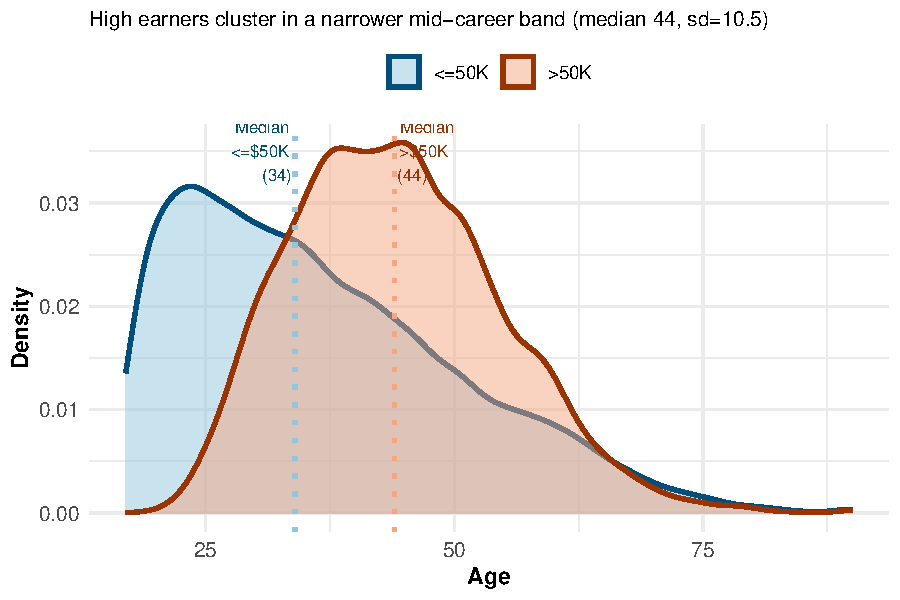
\includegraphics[keepaspectratio]{report_files/figure-pdf/age-density-1.pdf}}

High earners (\textgreater\$50K) have a median age of 44 with a standard
deviation of 10.5 years. Lower earners have a median of 34 and a
standard deviation of 14.0. The difference in spread --- not just center
--- is notable: the high-earning population is concentrated in a roughly
30--60 age band, with relatively few above 65 (where retirement reduces
labor force participation) and almost none below 25. Lower earners, by
contrast, are present in meaningful numbers from 17 upward and across a
full working life.

This pattern is consistent with what a career-trajectory model would
predict: high-earning positions require years of education and work
experience to reach, which compresses their age distribution into the
mid-career band. The younger left tail of the lower-earner distribution
is largely students, entry-level workers, and early-career adults who
have not yet reached income-earning years --- not adults stuck at low
wages across a full career.

\subsection{Trends}\label{trends}

\subsubsection{Education and the threshold that almost
matters}\label{education-and-the-threshold-that-almost-matters}

Education is the single strongest numeric predictor of income in this
dataset (correlation 0.335 with the binary outcome, the highest of any
numeric variable). But the relationship is not linear --- it has a
pronounced threshold shape.

\begin{Shaded}
\begin{Highlighting}[]
\NormalTok{p\_edu }\OtherTok{\textless{}{-}} \FunctionTok{readRDS}\NormalTok{(}\StringTok{"../data/processed/chart\_edu\_trend.rds"}\NormalTok{)}
\NormalTok{p\_edu}
\end{Highlighting}
\end{Shaded}

\pandocbounded{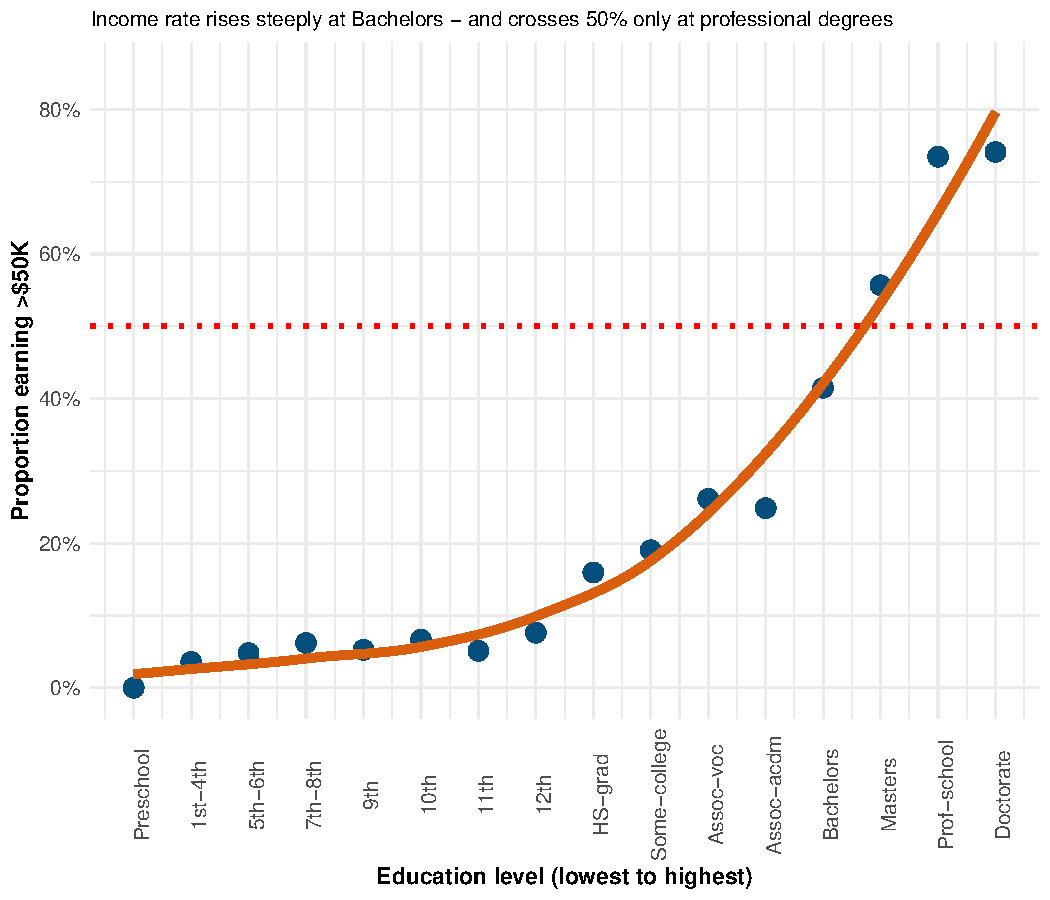
\includegraphics[keepaspectratio]{report_files/figure-pdf/education-trend-1.pdf}}

From Preschool through 12th grade, the income rate hovers below 8\%
across all levels --- the differences between, say, 9th grade and 11th
grade are small in absolute terms. At HS-grad the rate reaches 16\%, and
Some-college climbs to 19\%. Then the slope steepens sharply: Bachelors
jumps to 41.5\%, Masters to 55.7\%, and the 50\% majority threshold is
crossed only at Prof-school (73.4\%) and Doctorate (74.1\%).

The practical implication is a two-tier educational structure:
completing a bachelor's degree is a necessary-but-not-sufficient
condition for majority odds of high income, and every level below it
confers roughly similar low odds. The associate degrees (Assoc-voc:
26.1\%, Assoc-acdm: 24.8\%) sit roughly halfway between high school and
bachelor's --- meaningful but short of the bachelor's step change.

Note that education level is the variable, not years of education
completed; ``Prof-school'' refers to professional school credentials
(law, medicine, dentistry) rather than just 15 years of schooling, which
explains why its income rate (73.4\%) matches Doctorate (74.1\%) rather
than falling between Masters and Doctorate.

\subsection{Anomalies and Domain-Specific
Findings}\label{anomalies-and-domain-specific-findings}

\subsubsection{The gender income gap and what it actually
measures}\label{the-gender-income-gap-and-what-it-actually-measures}

The headline gender income gap in this dataset is substantial: 10.9\% of
women earn \textgreater\$50K, compared to 30.6\% of men --- a nearly
three-to-one ratio. Taken at face value, this would suggest severe pay
discrimination or occupational segregation.

Conditioning on marital status reveals a very different picture.

\begin{Shaded}
\begin{Highlighting}[]
\NormalTok{p\_gm }\OtherTok{\textless{}{-}} \FunctionTok{readRDS}\NormalTok{(}\StringTok{"../data/processed/chart\_gender\_marriage.rds"}\NormalTok{)}
\NormalTok{p\_gm}
\end{Highlighting}
\end{Shaded}

\pandocbounded{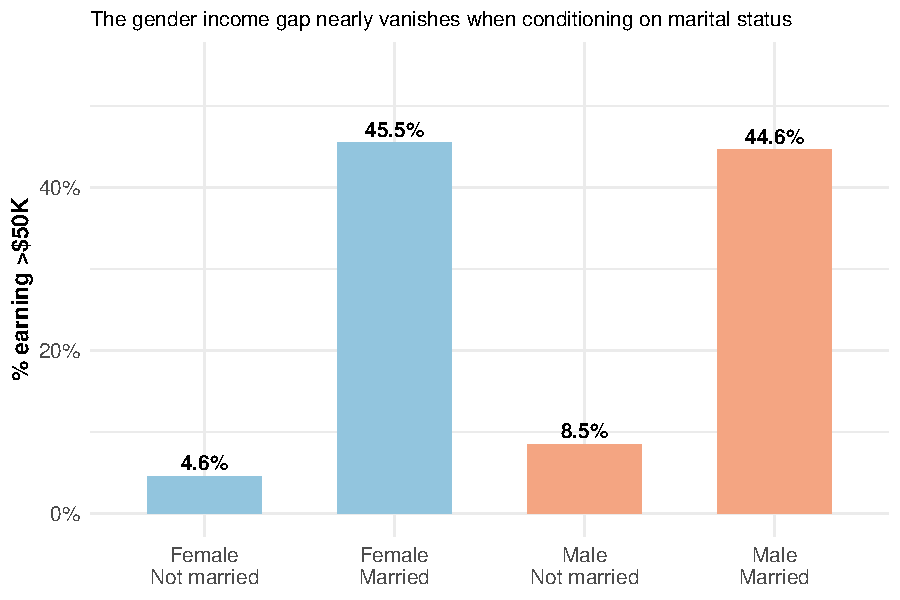
\includegraphics[keepaspectratio]{report_files/figure-pdf/gender-marriage-1.pdf}}

Among \textbf{married} respondents, the gap nearly vanishes: married
women earn \textgreater\$50K at a rate of \textbf{45.5\%}, essentially
identical to married men at \textbf{44.6\%}. Among non-married
respondents, the gap remains (female: 4.6\%, male: 8.5\%), but both
rates are much lower than the married rates.

This is a \textbf{selection effect, not an equal-pay story.} In the 1994
labor market, married women who were in the labor force at all were
heavily concentrated in professional and managerial roles --- the women
who stayed in full-time employment while married tended to be in exactly
the occupations that pay above \$50K. The aggregate 10.9\% female rate
is the average across all women in the sample, including large numbers
working part-time, in lower-wage sectors, or with career interruptions.
The aggregate number is real, but it measures who is in which
labor-force category, not wage discrimination between men and women
doing the same jobs.

What this data cannot say: whether women in the same role as men were
paid equally. But looking within credentials rather than within marital
status reveals that the picture is more complex than ``married women
earn as much as men.''

\textbf{Within credentials, the gap persists.} Among bachelor's degree
holders: female 20.9\% \textgreater\$50K vs.~male 50.4\% --- a 2.4x
differential. Among master's holders: female 33.4\% vs.~male 65.7\%.
Only at the doctoral level do the rates begin to converge (female 58.1\%
vs.~male 78.3\%). The external benchmark is consistent: the 1994 Census
P60-193 reports female-to-male earnings at 73\% for full-time year-round
workers overall, and specifically \$35,378 vs.~\$49,228 for bachelor's
or higher holders. Women with bachelor's degrees were earning 29\% below
the \$50K threshold on average; men with bachelor's degrees were
essentially at it. The married-female finding (45.5\%) reflects a highly
selected subgroup --- the women who remained in full-time professional
employment while married in 1994 were concentrated in the
highest-earning niches of each occupation. The broader picture is that
the credential-income relationship operated along a 70--30 fault line by
sex.

\subsubsection{Occupation: a structural income
floor}\label{occupation-a-structural-income-floor}

\begin{Shaded}
\begin{Highlighting}[]
\NormalTok{p\_occ }\OtherTok{\textless{}{-}} \FunctionTok{readRDS}\NormalTok{(}\StringTok{"../data/processed/chart\_occ\_lollipop.rds"}\NormalTok{)}
\NormalTok{p\_occ}
\end{Highlighting}
\end{Shaded}

\pandocbounded{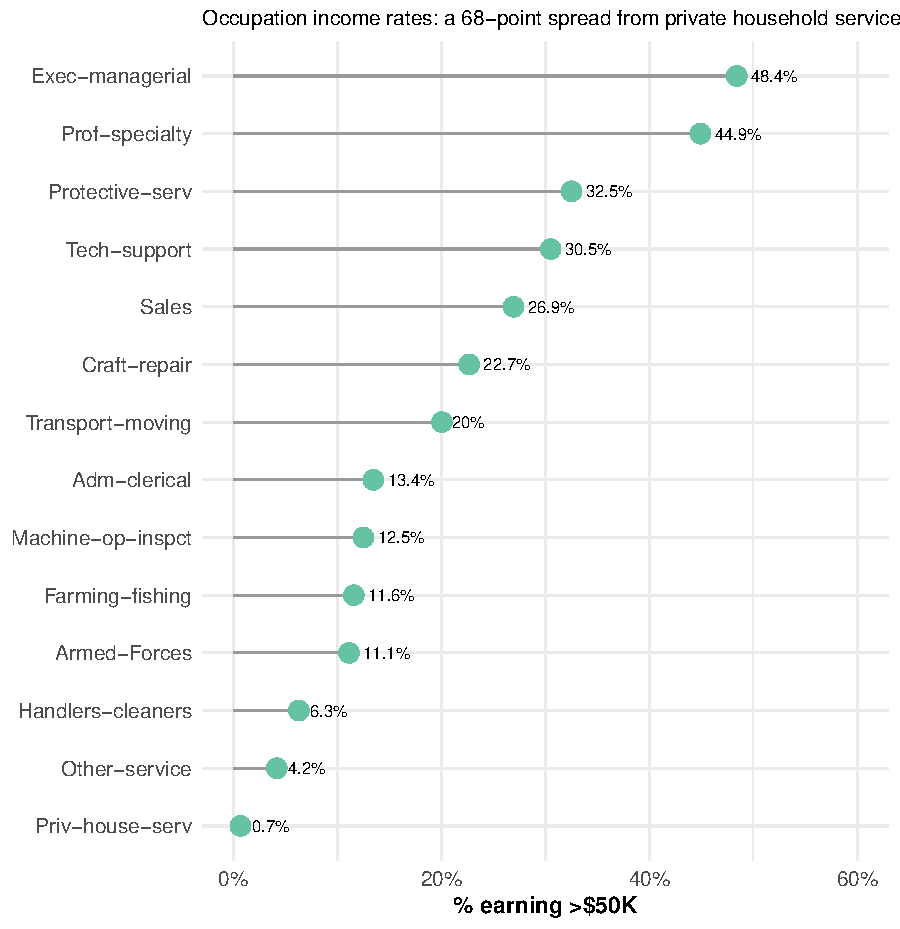
\includegraphics[keepaspectratio]{report_files/figure-pdf/occupation-ranking-1.pdf}}

Across 14 named occupations, the income rate spans 68 percentage points
--- from Priv-house-serv (private household service: 0.7\%) to
Exec-managerial (48.4\%). \textbf{None} of the 149 private household
service workers in this sample earn above \$50K. This is not a
statistical edge case --- it is the floor of the occupational structure,
where wages are constrained by the ability-to-pay of individual
households rather than corporate employment markets. The occupation acts
as a near-absolute income ceiling for the people in it.

The top two occupations (Exec-managerial and Prof-specialty) together
account for 8,206 respondents --- roughly 25\% of the sample --- and
both hover near or above 45\%. Below them is a large middle tier
(Protective-serv through Transport-moving, 20--32\%), then a sharp drop
into the administrative and service occupations (Adm-clerical through
Farming-fishing, 11--13\%), and a bottom cluster (Handlers-cleaners,
Other-service, Priv-house-serv) at single digits.

Occupation and education are correlated predictors --- workers in
higher-income occupations tend to have higher education levels. Neither
can be called the ``cause'' of income at this level of analysis; both
reflect accumulated structural position.

\subsubsection{Capital gains: investment income as a high-earner
signal}\label{capital-gains-investment-income-as-a-high-earner-signal}

Capital gains are, for most people in this sample, simply absent.

\begin{Shaded}
\begin{Highlighting}[]
\NormalTok{p\_cg }\OtherTok{\textless{}{-}} \FunctionTok{readRDS}\NormalTok{(}\StringTok{"../data/processed/chart\_capital\_gain.rds"}\NormalTok{)}
\NormalTok{p\_cg}
\end{Highlighting}
\end{Shaded}

\pandocbounded{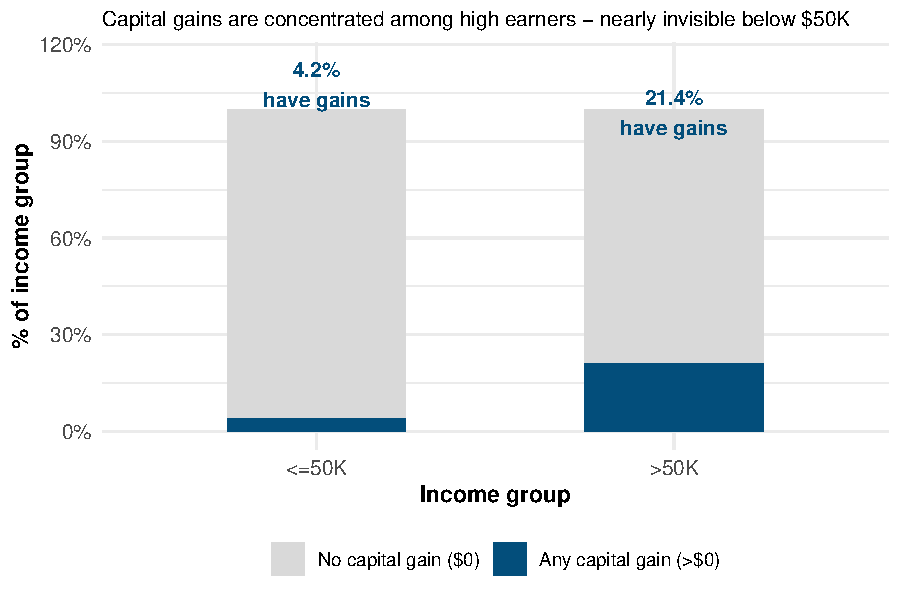
\includegraphics[keepaspectratio]{report_files/figure-pdf/capital-gains-1.pdf}}

\textbf{91.7\% of all respondents report \$0 in capital gains.} Among
the remaining 8.3\%, there is wide variation: the median non-zero gain
is \$7,896 among high earners and \$3,273 among lower earners. The
pattern reverses at the top: 2\% of high earners hit the \$99,999
reporting ceiling (suggesting actual gains well above that figure),
versus essentially zero among lower earners.

The five-fold difference in any-capital-gain prevalence (4.2\%
vs.~21.4\%) is the cleanest signal in the dataset that high income and
investment income co-occur --- people above the \$50K wage threshold are
also, at much higher rates, building wealth through investment returns.
This is not simply a case of people investing more because they have
more money left after expenses (though that is likely part of the
story); it also reflects differential access to investment vehicles,
financial literacy, and employer-offered stock programs, all of which
were concentrated in higher-income professional roles in 1994.

The \$99,999 top-code means that for high-earning investors, the true
scale of capital gains is unknown and potentially much larger than the
data shows. Any summary statistic for capital\_gain that includes the
censored rows should be read as a lower bound for those respondents.

\subsubsection{Race disparities: a coarse but real
signal}\label{race-disparities-a-coarse-but-real-signal}

Income rates vary substantially by race in this sample: Asian-Pacific
Islander (26.6\%) and White (25.6\%) respondents have nearly identical
rates; Black (12.4\%), American Indian/Eskimo (11.6\%), and Other
(9.2\%) respondents have rates roughly half as high. These are coarse
univariate numbers --- race interacts with occupation, education, and
nativity in ways that a single proportion cannot disentangle. The raw
disparity is real and worth naming, but the mechanism cannot be
established from a comparison of these proportions alone.

\section{Conclusion}\label{conclusion}

The 1994 CPS Adult dataset shows a labor market where high individual
income (\$50K, roughly equivalent to \$105,000 in today's dollars) was
relatively rare --- captured by 24\% of the working adults in the sample
--- and concentrated along three structural dimensions: educational
credentials, occupational sector, and career stage.

Education functions as a near-binary gate in this data. Below a
bachelor's degree, income rates stay in single digits regardless of
grade level completed; at the bachelor's degree, the rate jumps to 41\%;
and above it, the majority of credential-holders (Masters, Prof-school,
Doctorate) earn above the threshold. This is not a smooth gradient ---
it is a structural discontinuity that the labor market was enforcing
even in 1994, before credential inflation had raised the floor further.

Occupation reinforces this structure but does not simply duplicate it:
the 68-point spread between private household service (0.7\%) and
executive-managerial (48.4\%) reflects that sector matters independently
of individual qualifications. The workers at the bottom of the
occupational ranking are not simply less-educated workers --- they are
in roles where the entire wage structure is constrained by who is
paying.

The gender income gap story is more nuanced than the headline 3:1 ratio
suggests. Married women and married men in this sample earn above the
threshold at essentially identical rates (45.5\% vs.~44.6\%). The
aggregate gap is almost entirely a 1994 labor-force-participation story:
far fewer women were in the married-professional category than men. This
data cannot speak to whether men and women in the same role were paid
the same; it can say that among those who reached
professional-managerial roles and remained in the workforce while
married, the income outcome was remarkably symmetric.

The capital gains finding is the one that most clearly reveals something
about how wealth works rather than just how wages work. For 92\% of this
sample, investment income is absent. For high earners, it is present at
5x the rate of lower earners. Wage income and investment income do not
simply track each other --- they appear as distinct layers of the income
distribution, with the investment layer accessible primarily to those
who have already cleared the wage threshold.

\textbf{Representativeness caveats.} This is a 1994 cross-sectional
extract, and the US labor market has shifted substantially since: the
college wage premium has widened, the gig economy has reshaped workclass
categories, and the demographic composition of the workforce has
changed. The \$50K threshold, equivalent to roughly \$106K today (BLS
CPI-U), places this analysis in the upper-quartile income conversation,
not the median-income conversation. Any direct application of these
findings to current policy or workforce planning should first establish
whether the structural patterns have held, sharpened, or reversed.

One representativeness concern is specific to the sample itself,
independent of era: the dataset contains 33.1\% female respondents
against an actual 1994 female labor force share of 45.9\% (BLS EcoPro
Table 1). The fnlwgt weights would correct for this in a weighted
analysis; all income-by-sex comparisons in this report are unweighted
and thus based on a male-skewed sample. The specific magnitude of
gender-related findings should be read with this caveat in mind.

\subsection{Analysis Approach (Next
Phase)}\label{analysis-approach-next-phase}

The five findings above define the structural landscape of the dataset.
A natural next step is binary classification modeling --- predicting the
\textgreater\$50K label from the available features, with special
attention to whether the model reproduces or obscures the demographic
disparities surfaced here. Given the data quality issues identified
(top-coded capital\_gain, co-missing workclass/occupation), any modeling
pipeline would need explicit decisions about imputation strategy,
capital\_gain treatment, and whether fnlwgt sampling weights should be
incorporated.

\section{Technical Notes}\label{technical-notes}

\subsection{Reproducibility}\label{reproducibility}

\begin{itemize}
\tightlist
\item
  \textbf{Environment:} R 4.5.x, tidyverse 2.0.0, arrow 14.x
\item
  \textbf{To reproduce from raw data:}

  \begin{enumerate}
  \def\labelenumi{\arabic{enumi}.}
  \tightlist
  \item
    From the project root, run \texttt{Rscript\ R/01\_prep.R} --- loads
    raw data, applies column names, replaces \texttt{?} nulls, writes
    \texttt{data/processed/adult\_clean.parquet}
  \item
    Run \texttt{Rscript\ R/02\_phase1\_tables.R} --- writes Phase 1
    summary tables as \texttt{.rds} to \texttt{data/processed/}
  \item
    Run \texttt{Rscript\ R/03\_charts.R} --- builds all chart objects
    and saves as \texttt{.rds} to \texttt{data/processed/}; also exports
    standalone PNGs to \texttt{output/figures/}
  \item
    Render this report: \texttt{quarto\ render\ output/report.qmd}
  \end{enumerate}
\item
  The report loads cached objects from \texttt{data/processed/} --- it
  does not re-read \texttt{data/raw/} directly.
\end{itemize}

\subsection{References}\label{references}

\begin{enumerate}
\def\labelenumi{\arabic{enumi}.}
\tightlist
\item
  US Census Bureau. \emph{Income, Poverty, and Valuation of Noncash
  Benefits: 1994.} Current Population Reports P60-189, 1996. Source of
  1994 income medians by sex and education.
\item
  US Census Bureau. \emph{Money Income in the United States: 1995.}
  Current Population Reports P60-193, 1996. Source of the female-to-male
  earnings ratio (\textasciitilde73\%) for full-time year-round workers.
\item
  Bureau of Labor Statistics. \emph{Employment Projections --- Table 1:
  Civilian labor force by age, gender, race, and ethnicity, 1994--2024.}
  bls.gov/news.release/ecopro.t01.htm. Source of 1994 labor force racial
  and sex composition benchmarks.
\item
  Bureau of Labor Statistics. \emph{Consumer Price Index for All Urban
  Consumers (CPI-U).} Annual average 1994: 148.2; 2024: 313.7. Source of
  inflation conversion (\$50K in 1994 ≈ \$105,800 in 2024).
\item
  Social Security Administration. \emph{National Average Wage Index
  Series.} ssa.gov/oact/cola/awiseries.html. Source of 1994 national
  average wage: \$23,754.
\item
  National Center for Education Statistics. \emph{Digest of Education
  Statistics 1996, Table 375.} Median earnings by education level and
  sex, 1994 full-time year-round workers.
\item
  National Center for Education Statistics. \emph{Digest of Education
  Statistics 1995, Table 371.} Unemployment rates by education level,
  1994.
\item
  UCI Machine Learning Repository. \emph{Adult Data Set.}
  archive.ics.uci.edu/ml/datasets/adult --- dataset column documentation
  only; not an external grounding source.
\item
  Becker, Barry and Kohavi, Ronny. \emph{Scaling Up the Accuracy of
  Naive-Bayes Classifiers: A Decision-Tree Hybrid.} KDD-96, 1996. ---
  original dataset publication; cited for provenance only.
\end{enumerate}




\end{document}
